\documentclass[tikz,border=6pt]{standalone}
\usepackage{tikz}
\usetikzlibrary{arrows.meta,positioning,shapes.geometric}

\definecolor{kmblue}{RGB}{0,56,116}
\definecolor{apcol}{RGB}{180,40,40}
\definecolor{rtgreen}{RGB}{30,130,60}
\definecolor{rscol}{RGB}{100,80,160}

\begin{document}
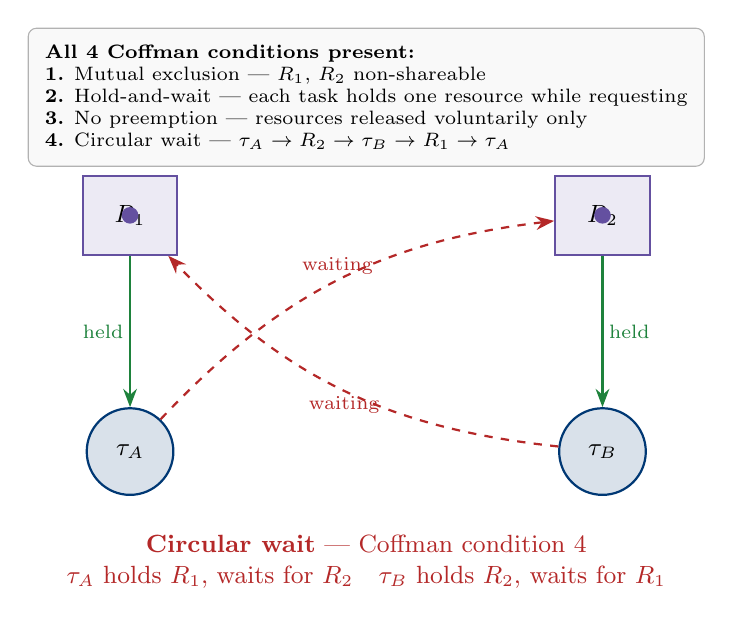
\begin{tikzpicture}[
  task/.style={circle, draw=kmblue, fill=kmblue!15, thick,
               minimum size=1.1cm, font=\small\bfseries},
  res/.style={rectangle, draw=rscol, fill=rscol!12, thick,
              minimum width=1.2cm, minimum height=1.0cm, font=\small\bfseries},
  assign/.style={->, >=Stealth, thick, rtgreen},   % resource → task
  request/.style={->, >=Stealth, thick, apcol, dashed},  % task → resource
  label/.style={font=\scriptsize, inner sep=2pt},
]

% Nodes
\node[task] (tA) at (0,0)   {$\tau_A$};
\node[task] (tB) at (6,0)   {$\tau_B$};
\node[res]  (R1) at (0,3)   {$R_1$};
\node[res]  (R2) at (6,3)   {$R_2$};

% Dot inside resource box = instance held
\fill[rscol] (0,3) circle (3pt);
\fill[rscol] (6,3) circle (3pt);

% Assignment edges (resource → task, held)
\draw[assign] (R1) -- node[left, label]{held} (tA);
\draw[assign] (R2) -- node[right, label]{held} (tB);

% Request edges (task → resource, waiting)
\draw[request] (tA) to[bend left=20]
  node[above, label, apcol]{waiting} (R2);
\draw[request] (tB) to[bend left=20]
  node[below, label, apcol]{waiting} (R1);

% Circular wait annotation
\node[font=\small, apcol, align=center] at (3,-1.4)
  {\textbf{Circular wait} — Coffman condition 4\\
   $\tau_A$ holds $R_1$, waits for $R_2$\quad
   $\tau_B$ holds $R_2$, waits for $R_1$};

% Coffman conditions callout
\node[draw=gray!60, rounded corners=3pt, fill=gray!5,
      font=\scriptsize, align=left, inner sep=6pt] at (3,4.5)
{%
  \textbf{All 4 Coffman conditions present:}\\
  \textbf{1.} Mutual exclusion — $R_1$, $R_2$ non-shareable\\
  \textbf{2.} Hold-and-wait — each task holds one resource while requesting\\
  \textbf{3.} No preemption — resources released voluntarily only\\
  \textbf{4.} Circular wait — $\tau_A \to R_2 \to \tau_B \to R_1 \to \tau_A$%
};

\end{tikzpicture}
\end{document}
